\section{Random Deployment}
\label{sec:random_deployment}

Advanced reactor concepts, like the ones outlined in this thesis, are often
designed for use cases ranging from industrial steam production to microgrid
integration. Reactor deployment is a complex problem that requires a nuanced understanding of the energy market, regulatory environment, intended use of the technology, and the technical capabilities of the reactor.

This random deployment is a proxy for the complexity of the real-world problem; however, it does not include the nuance of how individual
deployments meet an end user's needs, which will drive the strategic decisions
that utilities and ratepayers behind the meter make in their reactor choices.
The random deployment scheme has the potential to capture some of the
complexities in overall market development, but the extent to which it captures these details is not explored in this thesis.

The random deployment scheme is implemented by randomly selecting reactors from the list of deployable reactors until the demand is covered. Figure \ref{fig:random_diagram} illustrates this scheme, which shows the single loop in the logic from the top down. There is an irreducible demand that cannot be met because the power capacity is assumed to be constant. At its best, the random deployment scheme will meet the demand but has the potential to fall short of the demand by one of the smallest capacity reactors. This thesis implements a rough random case that deploys until the randomly selected reactor exceeds the demand to reduce the computational cost. This rough approximation is coupled with the greedy deployment scheme in the initially random, greedy deployment scheme in Section \ref{sec:initially_random_greedy}.

\begin{figure}[H]
  \centering
  \begin{tikzpicture}[node distance = 2.5cm, auto]
    % Place nodes
    \node [block] (init) {\textbf{Initialize demand.}};
    \node [block, below of=init] (check) {\textbf{Is there demand?}};
    \node [block, below of=check, node distance=2.5cm] (evaluate) {\textbf{Randomly deploy one reactor.}};
    \node [block, below of=evaluate] (update) {\textbf{Update demand.}};
    \node [block, left of=check, node distance=3.5cm] (stop) {\textbf{Next time step.}};
    % Draw edges
    \path [line, line width=0.6mm] (init) -- (check);
    \path [line, line width=0.6mm] (check) -- node {\textbf{Yes}} (evaluate);
    \path [line, line width=0.6mm] (evaluate) -- (update);
    \path [line, line width=0.6mm] (check) -- node {\textbf{No}}(stop);
    \draw[->, line width=0.6mm] (update) edge[bend right=65] node[right]{} (check);
  \end{tikzpicture}
  \caption{The random deployment diagram shows the method by which this scheme selects reactors at each time step.}
  \label{fig:random_diagram}
\end{figure}

% \begin{figure}[H]
%     \centering
%     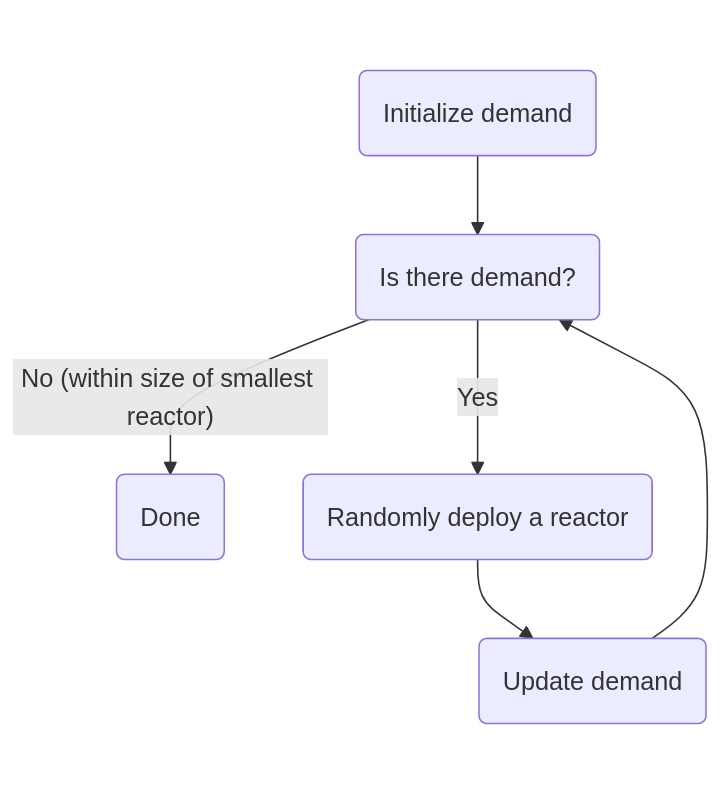
\includegraphics[scale=0.3]{images/schemes/random_diagram.png}
%     \caption{Random deployment diagram.}
%     \label{fig:random_diagram}
% \end{figure}

The seed, which was set to 20240527121205 for every run for this scheme, for
the random number generator is set by the date and time of the simulation,
which allows for the reproducibility of the results. This scheme is a proxy for
aggregate decisions by actors and would fail to reliably capture individual
actor decisions. This scheme is most useful for scenarios or timescales where
there is a high degree of uncertainty in the deployment of reactors.


\subsection{Number of Reactors}
\label{sec:random_reactors}

As discussed in Section \ref{sec:greedy_reactors}, the difference between the \textit{no growth} and \textit{double by 2050} scenarios in Figures \ref{fig:random_mf_reactors} and \ref{fig:random_of_reactors} is that the \textit{double by 2050} scenario requires new reactors to be deployed immediately during the transition. A consequence of the random reactor deployment scheme is that the reactors in Figures \ref{fig:random_mf_ng_reactors} and \ref{fig:random_mf_d2_reactors} grows similarly over time as they are sampled for deployment. This scheme has the potential to stochastically capture the complexity of deploying reactors in the real world but likely represents an extreme where utilities are not narrowing in on a single reactor design to reduce deployment costs.

% Show total number of reactors multi-fuel
\begin{figure}[H]
    \subfloat[No Growth. \label{fig:random_mf_ng_reactors}]{%
      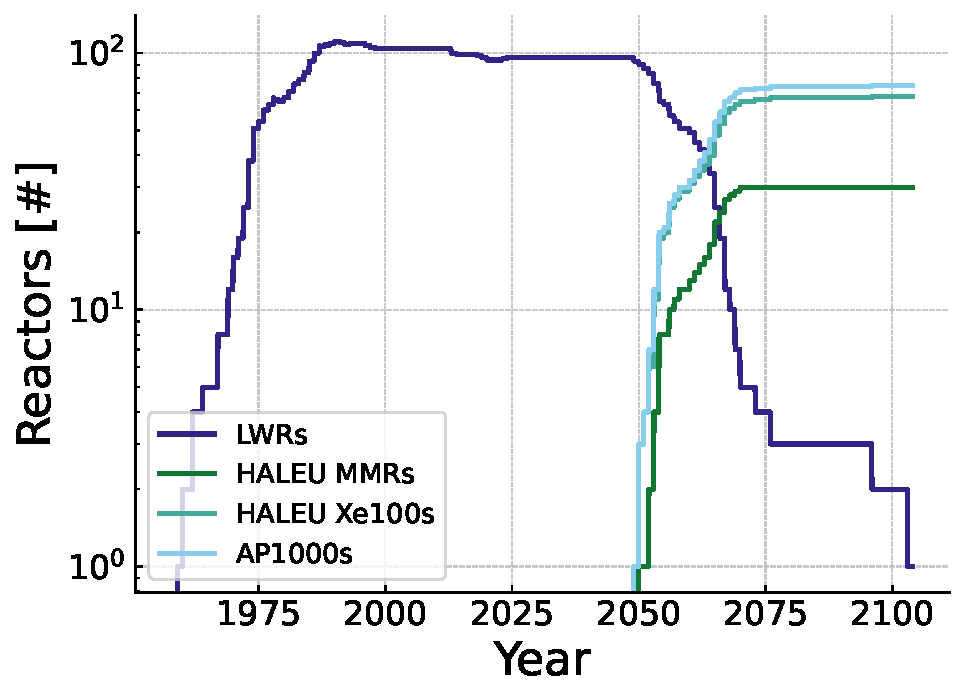
\includegraphics[width=0.495\textwidth]{images/results/reactors/multi_drng_reactors.pdf}
   }
    \hfill
    \subfloat[Double. \label{fig:random_mf_d2_reactors}]{%
      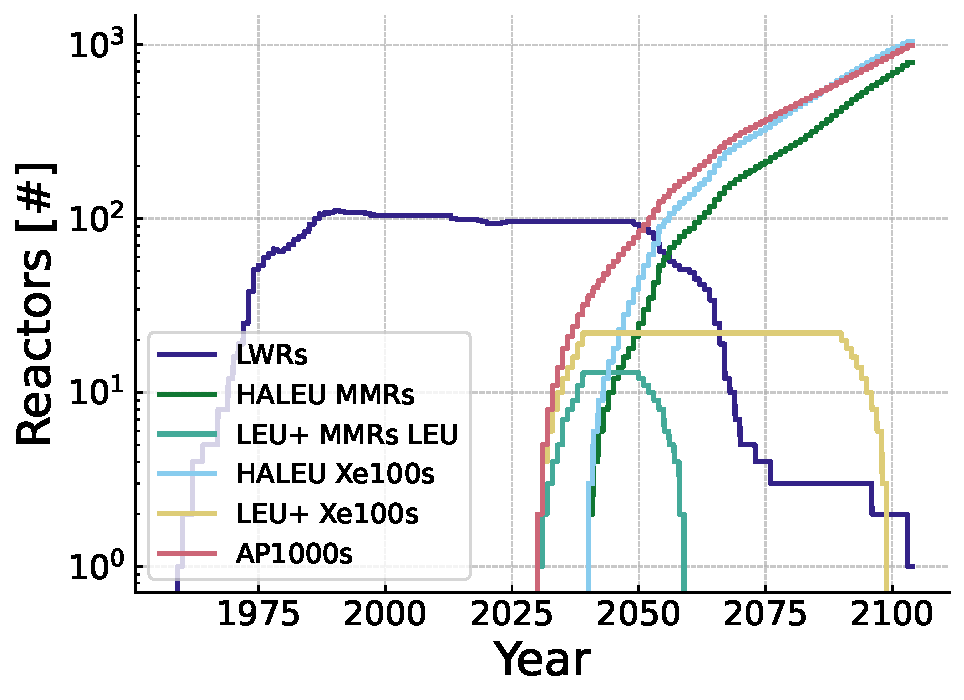
\includegraphics[width=0.495\textwidth]{images/results/reactors/multi_dr2_reactors.pdf}
   }
    \caption{Multiple fuels random reactor deployment.}
    \label{fig:random_mf_reactors}
  \end{figure}

% talk about the rate of deployment

% talk about the context of expanding energy needs

% talk about the workers

\begin{figure}[H]
    \subfloat[No Growth. \label{fig:random_of_ng_reactors}]{%
      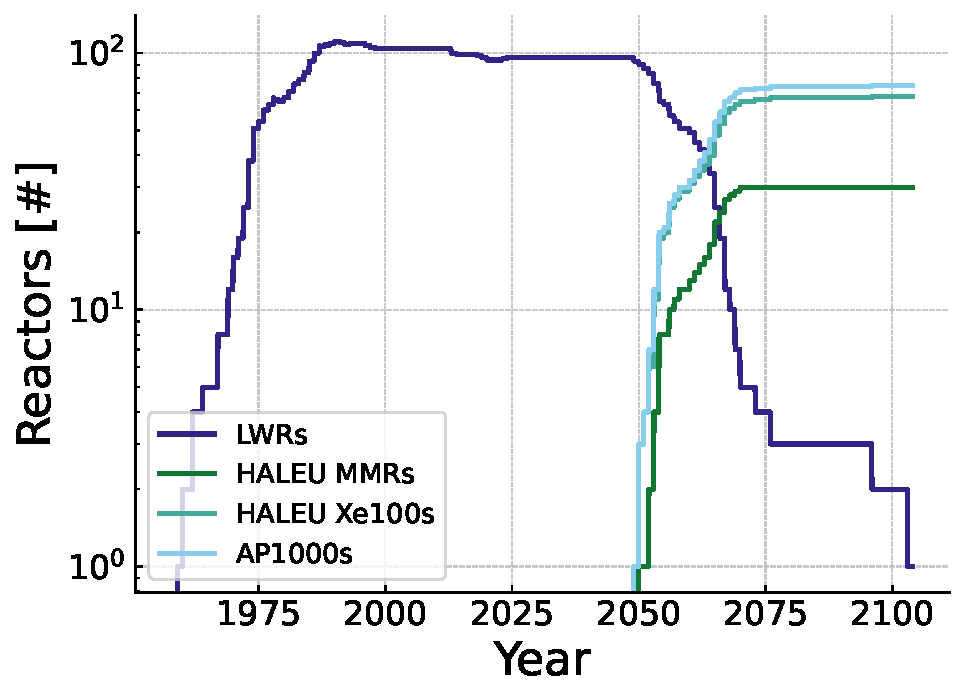
\includegraphics[width=0.495\textwidth]{images/results/reactors/one_drng_reactors.pdf}
   }
    \hfill
    \subfloat[Double. \label{fig:random_of_d2_reactors}]{%
      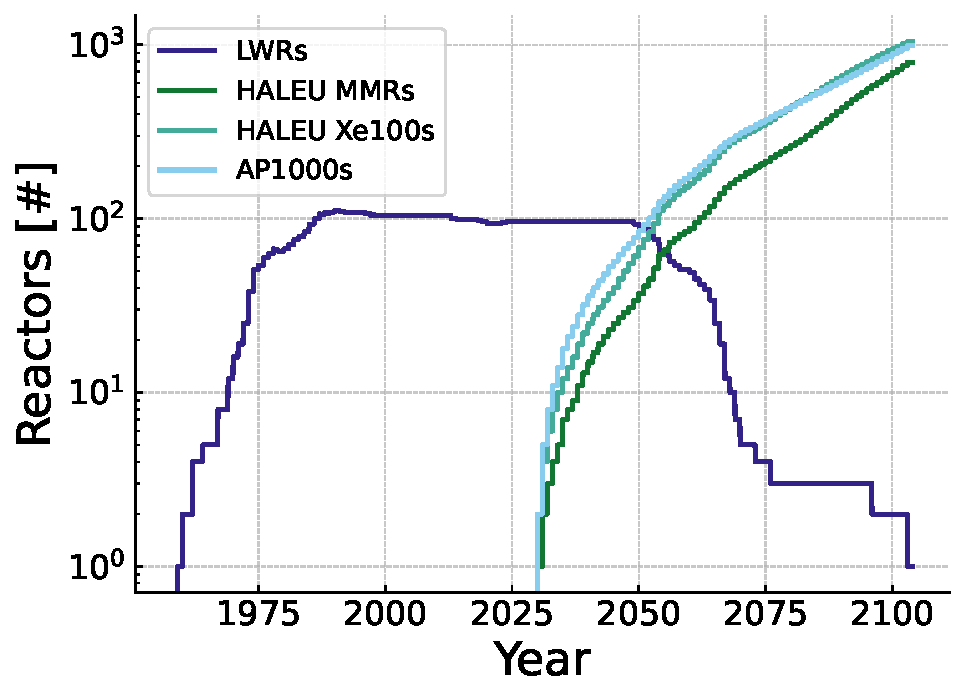
\includegraphics[width=0.495\textwidth]{images/results/reactors/one_dr2_reactors.pdf}
   }
    \caption{Single-fuel random reactor deployment.}
    \label{fig:random_of_reactors}
  \end{figure}


Table \ref{tab:random_reac_avg} shows the average total number of reactors for the \textit{no growth} and \textit{double by 2050} scenarios in the single and multi-fuel enrichment deployments. There is a 740\% increase in the AP1000s deployed from the \textit{no growth} scenario to the \textit{double by 2050} scenario. The \gls{xe} reactors show a 249\% increase, while the \gls{mmr} reactors show a 62\% increase in the reactors deployed from the \textit{no growth} scenario to the \textit{double by 2050} scenario in the single-fuel enrichment deployment. Unlike the reactor deployment under the greedy scheme in Section \ref{sec:greedy_reactors} and the initially random then greedy scheme in Section \ref{sec:rand_greed_reactors}, the random deployment scheme results for the single-fuel and multi-fuel enrichment deployments are not the same.

In the multi-fuel enrichment deployment, the AP1000 reactors show a 660\% increase in the reactors deployed from the \textit{no growth} scenario to the \textit{double by 2050} scenario. The \gls{xe} reactors show a 746\% increase, while the \gls{mmr} reactors show an 1138\% increase in the reactors deployed from the \textit{no growth} scenario to the \textit{double by 2050} scenario.

\begin{table}[H]
    \centering
    \caption{Average random total operating reactors by design.}
    \label{tab:random_reac_avg}
    \begin{tabular}{l c c c c}
       \toprule
       Scenario & \shortstack{No Growth,\\ Single} & \shortstack{No Growth,\\ Multiple} & \shortstack{Double,\\ Single} & \shortstack{Double,\\ Multiple}  \\
       \midrule
       \gls{haleu} fueled \glspl{mmr} & 131.613 & \textcolor{white}{0}17.267  & 213.707 & 210.24  \\
       \gls{leup} fueled \glspl{mmr}  & --      & --      & --      & \textcolor{white}{00}3.467   \\
       \gls{haleu} fueled \glspl{xe}  & \textcolor{white}{0}94.04   & \textcolor{white}{0}38.813  & 328.173 & 310.573 \\
       \gls{leup} fueled \glspl{xe}   & --      & --      & --      & \textcolor{white}{0}17.6    \\
       \gls{leu} fueled AP1000s       & \textcolor{white}{0}38.667  & \textcolor{white}{0}42.72   & 324.68  & 324.68  \\
       \bottomrule
    \end{tabular}
\end{table}




\subsection{SWU Results}
\label{sec:random_swu}

Figure \ref{fig:swu_yearly_random} visualizes the yearly \gls{swu} demand periodically spike as reactors begin operation in the depicted \textit{no growth} scenario around 2050. The \gls{swu} demand for the AP1000 \gls{leu} rises above the other two reactors where the demand from \glspl{xe} overlaps heavily with the demand from \glspl{mmr}. This trend is exacerbated in the \textit{double by 2050} scenarios shown in Figures \ref{fig:greedy_mf_d2_swu} and \ref{fig:greedy_of_d2_swu}, where the \gls{swu} for AP1000 \gls{leu} fuel rises quickly and eventually exceeds the total \gls{swu} for the existing fleet.


% talk about the SWU demand

% show the total SWU demand
\begin{figure}[H]
    \centering
    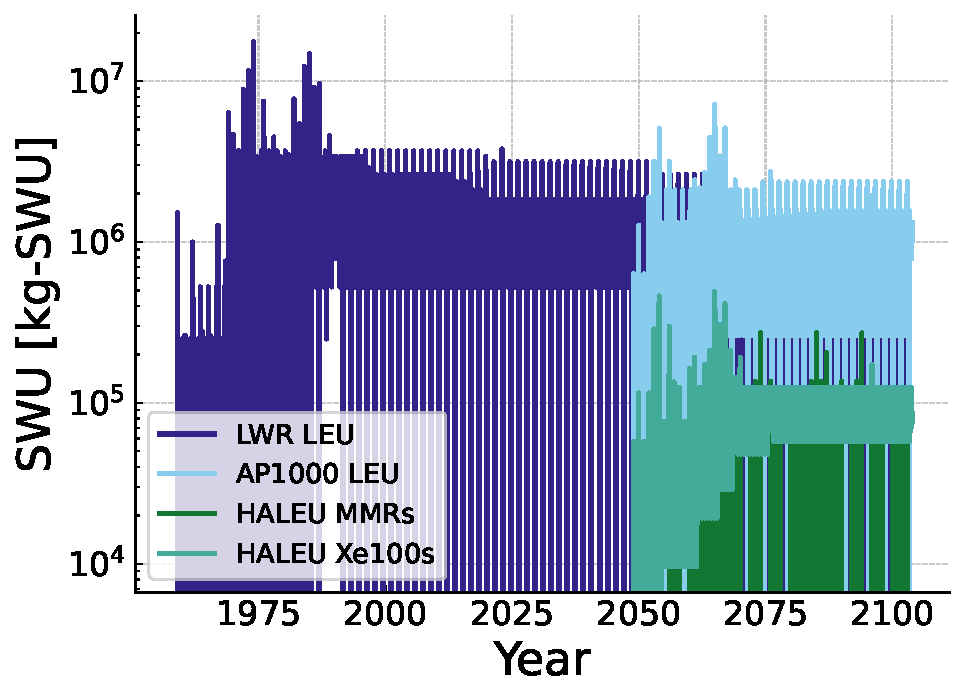
\includegraphics[scale=0.7]{images/results/swu/multi_drng_swu_by_fuel.pdf}
    \caption{Random reactor yearly SWU demand.}
    \label{fig:swu_yearly_random}
\end{figure}

As the features of the yearly data are regular, dictated by the cycles of the
reactors, and overlapping, Figures \ref{fig:random_mf_swu} and \ref{fig:random_of_swu} visualize the total cumulative \gls{swu} demand.


\begin{figure}[H]
  \subfloat[No Growth. \label{fig:random_mf_ng_swu}]{%
    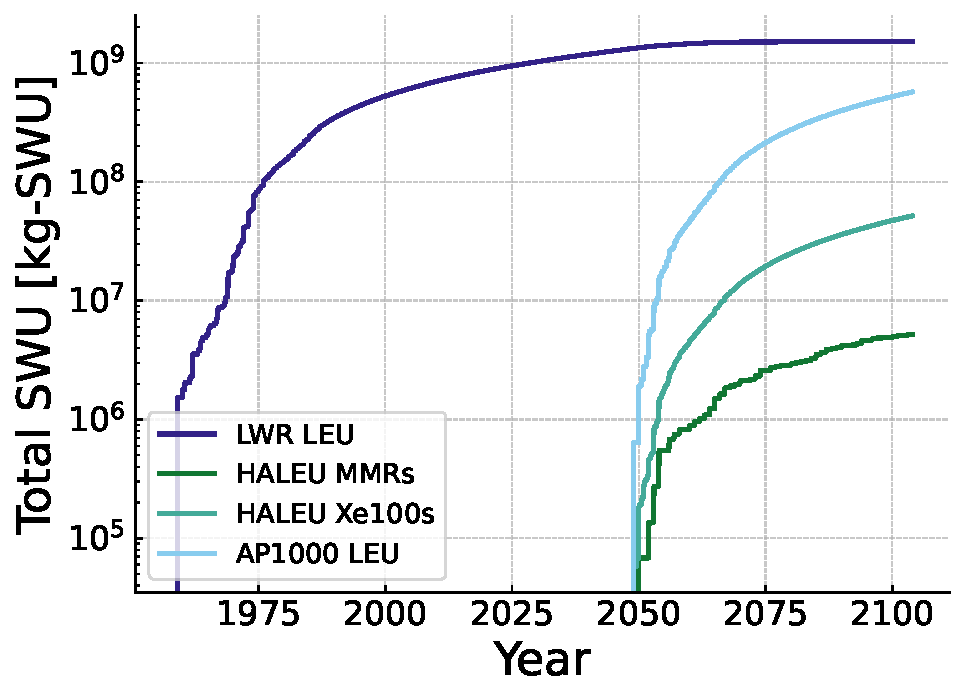
\includegraphics[width=0.495\textwidth]{images/results/swu/multi_drng_swu_cumulative_by_fuel.pdf}
 }
  \hfill
  \subfloat[Double. \label{fig:random_mf_d2_swu}]{%
    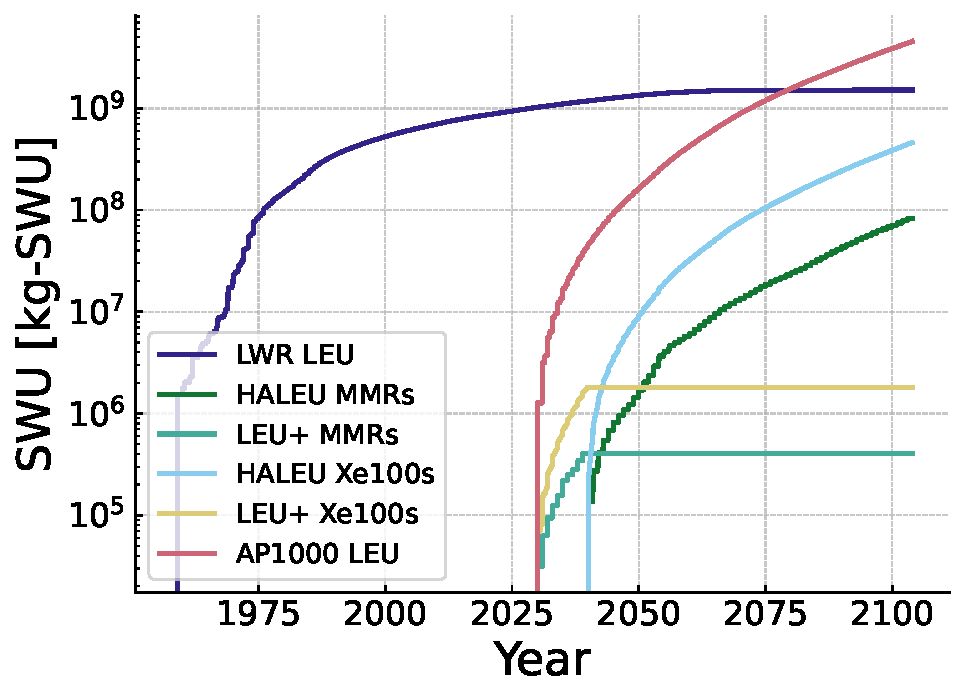
\includegraphics[width=0.495\textwidth]{images/results/swu/multi_dr2_swu_cumulative_by_fuel.pdf}
 }
  \caption{Random reactor multi-fuel SWU.}
  \label{fig:random_mf_swu}
\end{figure}

% talk about international trade

\begin{figure}[H]
    \subfloat[No Growth. \label{fig:random_of_ng_swu}]{%
      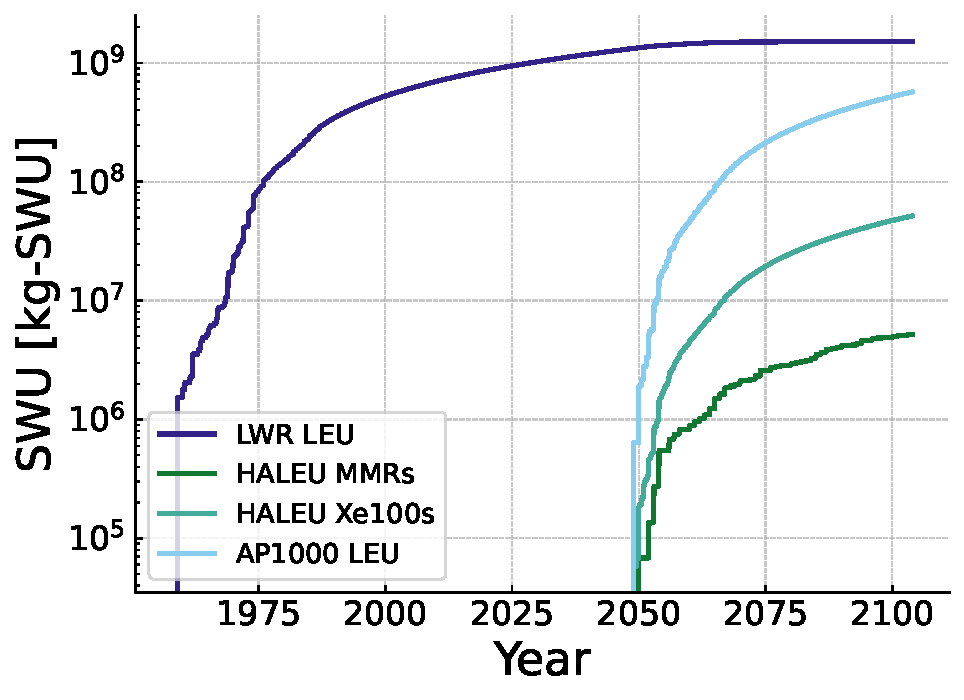
\includegraphics[width=0.495\textwidth]{images/results/swu/one_drng_swu_cumulative_by_fuel.pdf}
   }
    \hfill
    \subfloat[Double. \label{fig:random_of_d2_swu}]{%
      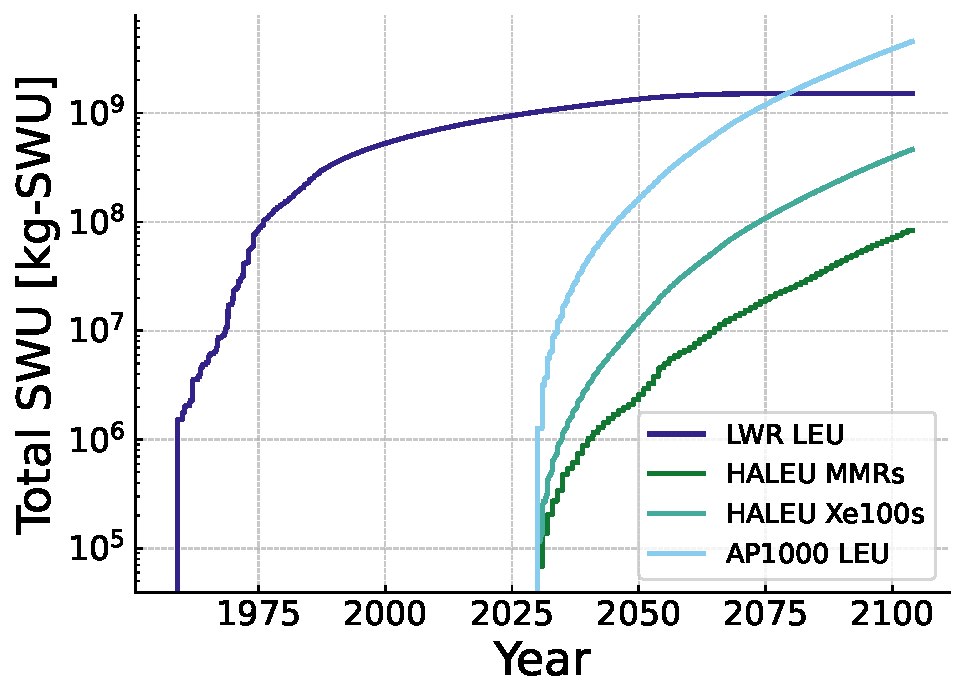
\includegraphics[width=0.495\textwidth]{images/results/swu/one_dr2_swu_cumulative_by_fuel.pdf}
   }
    \caption{Random reactor single-fuel SWU.}
    \label{fig:random_of_swu}
\end{figure}


Table \ref{tab:random_swu_avg} shows the average total yearly \gls{swu} demand for the \textit{no growth} and \textit{double by 2050} scenarios in the single and multi-fuel enrichment deployments under the random deployment scheme. The \gls{xe} reactors show a 796\% increase in the average total yearly \gls{swu} demand from the \textit{no growth} scenario to the \textit{double by 2050} scenario in the single-fuel enrichment deployment. The \glspl{mmr} show a 1511\% increase in the average total yearly \gls{swu} demand from the \textit{no growth} scenario to the \textit{double by 2050} scenario in the single-fuel enrichment deployment. The AP1000 reactors show a 697\% increase in the average total yearly \gls{swu} demand from the \textit{no growth} scenario to the \textit{double by 2050} scenario in the single-fuel enrichment deployment.

\begin{table}[H]
    \centering
    \caption{Average random yearly SWU by design in tonnes of \gls{swu}.}
    \label{tab:random_swu_avg}
    \begin{tabular}{l c c c c}
       \toprule
       Scenario & \shortstack{No Growth,\\ Single} & \shortstack{No Growth,\\ Multiple} & \shortstack{Double,\\ Single} & \shortstack{Double,\\ Multiple}  \\
       \midrule
       \gls{mmr} \gls{haleu}   & \textcolor{white}{000}5.756   & \textcolor{white}{000}5.756   & \textcolor{white}{00}92.703    & \textcolor{white}{00}91.719   \\
       \gls{mmr} \gls{leup}    & --      & --      & --       & \textcolor{white}{000}0.453    \\
       \gls{xe} \gls{haleu}    & \textcolor{white}{00}57.327  & \textcolor{white}{00}57.327  & \textcolor{white}{0}513.746  & \textcolor{white}{0}510.388  \\
       \gls{xe} \gls{leup}     & --      & --      & --       & \textcolor{white}{000}2.021    \\
       AP1000 \gls{leu}        & \textcolor{white}{0}634.554 & \textcolor{white}{0}634.554 & 5050.323 & 5050.323 \\
       \bottomrule
    \end{tabular}
\end{table}





\subsection{Fresh Fuel Results}
\label{sec:random_fresh}

% talk about the types of fuel
Figures \ref{fig:random_mf_fresh} and \ref{fig:random_of_fresh} show the fresh fuel demand for the reactors in the \textit{no growth} and \textit{double by 2050} scenarios. The fresh fuel curves in each scenario follow the same pattern as the reactor deployment curves from Figures \ref{fig:random_mf_reactors} and \ref{fig:random_of_reactors}, as \cyclus supplies fuel to each of the reactors as they deploy.

% show total fresh fuel

\begin{figure}[H]
    \subfloat[No Growth. \label{fig:random_mf_ng_fresh}]{%
      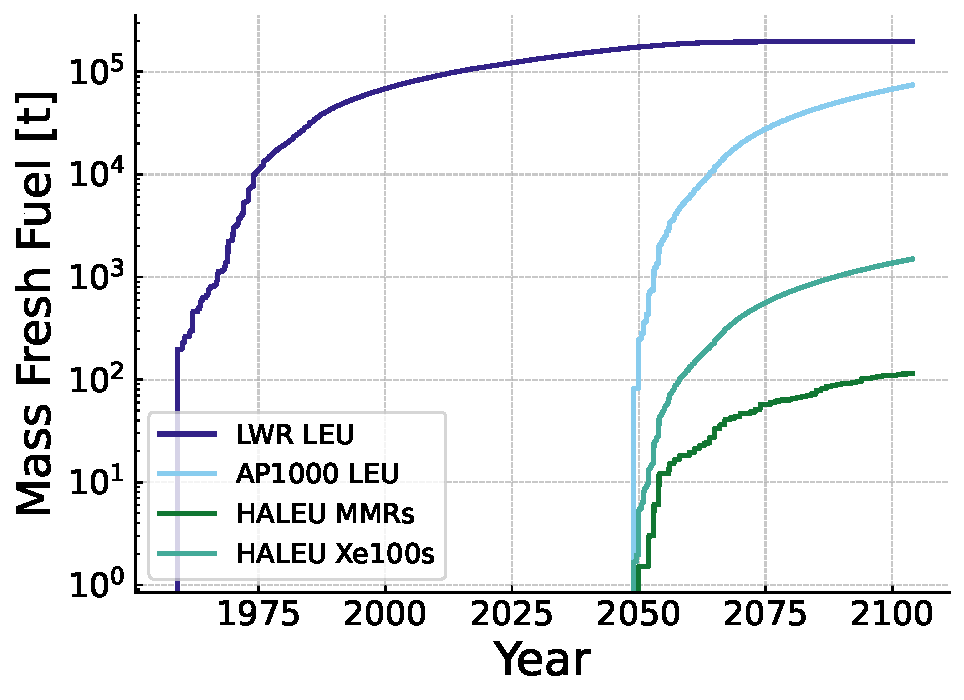
\includegraphics[width=0.495\textwidth]{images/results/fresh/multi_drng_fresh_fuel_cumulative_by_fuel.pdf}
   }
    \hfill
    \subfloat[Double. \label{fig:random_mf_d2_fresh}]{%
      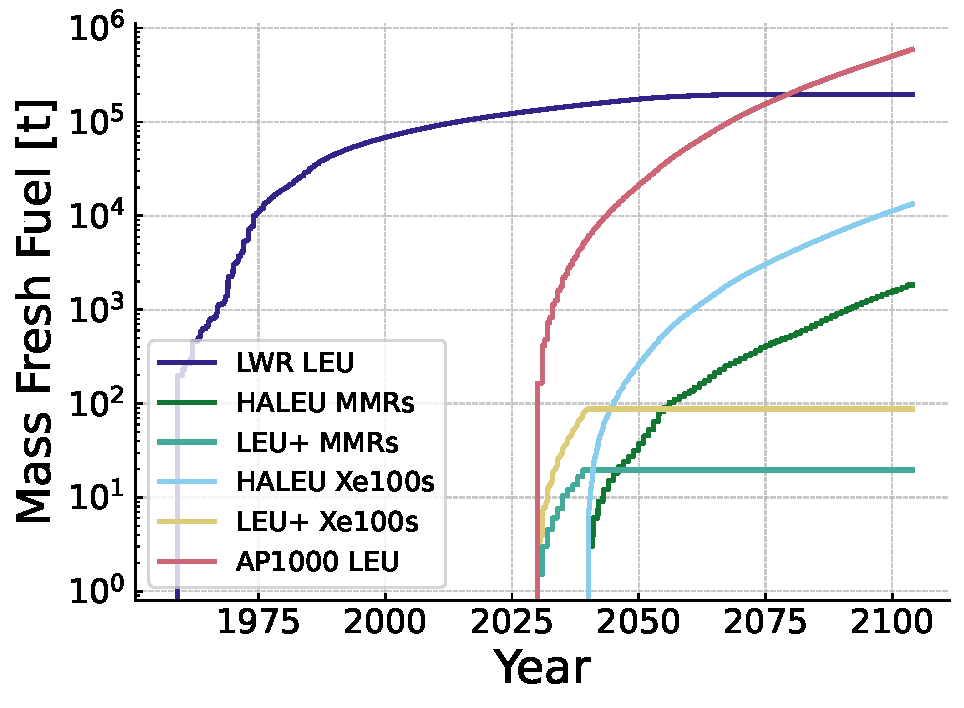
\includegraphics[width=0.495\textwidth]{images/results/fresh/multi_dr2_fresh_fuel_cumulative_by_fuel.pdf}
   }
    \caption{Random multi fresh fuel demanded.}
    \label{fig:random_mf_fresh}
  \end{figure}

% talk about transportation of fuel


\begin{figure}[H]
    \subfloat[No Growth. \label{fig:random_of_ng_fresh}]{%
      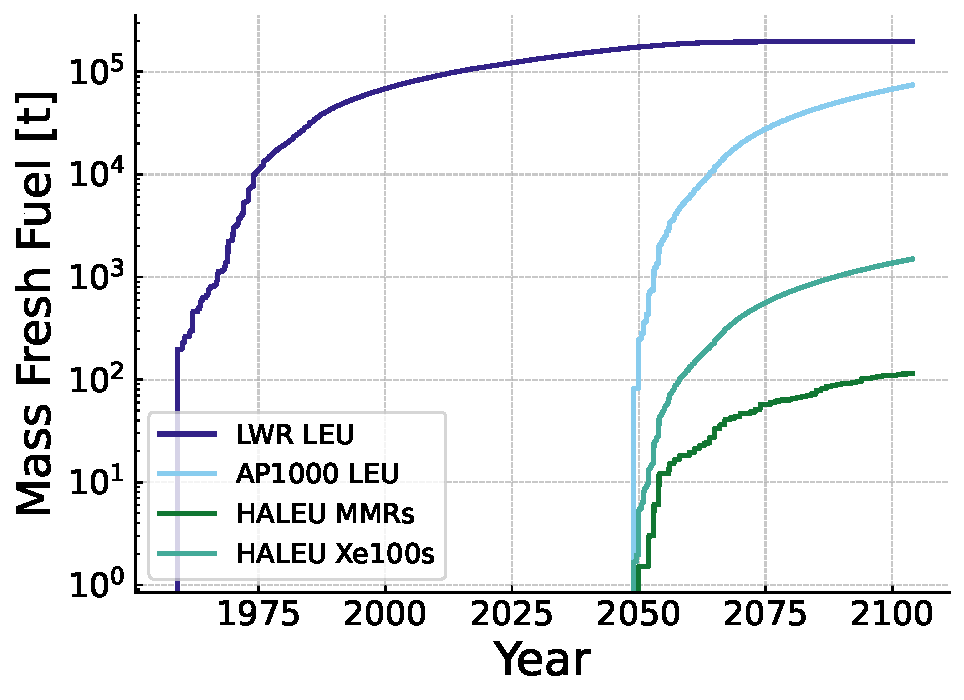
\includegraphics[width=0.495\textwidth]{images/results/fresh/one_drng_fresh_fuel_cumulative_by_fuel.pdf}
   }
    \hfill
    \subfloat[Double. \label{fig:random_of_d2_fresh}]{%
      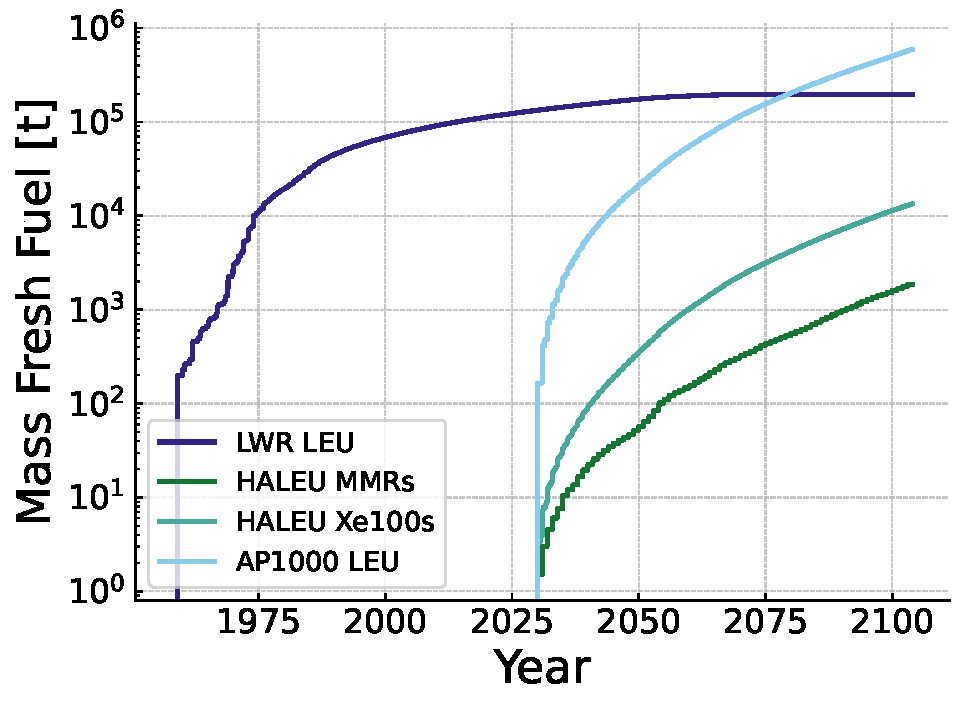
\includegraphics[width=0.495\textwidth]{images/results/fresh/one_dr2_fresh_fuel_cumulative_by_fuel.pdf}
   }
    \caption{Random single fresh fuel demanded.}
    \label{fig:random_of_fresh}
\end{figure}

Table \ref{tab:random_fresh_avg} shows the average total yearly fresh fuel for the \textit{no growth} and \textit{double by 2050} scenarios in the single and multi-fuel enrichment deployments under the random deployment scheme. The \gls{xe} reactors show a 796\% increase in the average total yearly fresh fuel from the \textit{no growth} scenario to the \textit{double by 2050} scenario in the single-fuel enrichment deployment. The \gls{mmr} reactors show a 1505\% increase in the average total yearly fresh fuel from the \textit{no growth} scenario to the \textit{double by 2050} scenario in the single-fuel enrichment deployment. The AP1000 reactors show a 696\% increase in the average total yearly fresh fuel from the \textit{no growth} scenario to the \textit{double by 2050} scenario in the single-fuel enrichment deployment.

\begin{table}[H]
    \centering
    \caption{Average random yearly fresh fuel by design in tonnes.}
    \label{tab:random_fresh_avg}
    \begin{tabular}{l c c c c}
       \toprule
       Scenario & \shortstack{No Growth,\\ Single} & \shortstack{No Growth,\\ Multiple} & \shortstack{Double,\\ Single} & \shortstack{Double,\\ Multiple}  \\
       \midrule
       \gls{mmr} \gls{haleu}   & \textcolor{white}{00}0.128    & \textcolor{white}{00}0.128   & \textcolor{white}{00}2.055    & \textcolor{white}{00}2.033    \\
       \gls{mmr} \gls{leup}    & --       & --      & --       & \textcolor{white}{00}0.107    \\
       \gls{xe} \gls{haleu}    & \textcolor{white}{00}1.663    & \textcolor{white}{00}1.663   & \textcolor{white}{0}14.904   & \textcolor{white}{0}14.806   \\
       \gls{xe} \gls{leup}     & --       & --      & --       & \textcolor{white}{00}0.022    \\
       AP1000 \gls{leu}        & \textcolor{white}{0}82.512   & \textcolor{white}{0}82.512  & 656.698  & 656.698  \\
       \bottomrule
    \end{tabular}
\end{table}





\subsection{Used Fuel Results}
\label{sec:random_used}

Figures \ref{fig:random_mf_used} and \ref{fig:random_of_used} depict the used fuel accumulation for the reactors in the \textit{no growth} and \textit{double by 2050} scenarios. The used fuel curves in each scenario follow the reactor deployment curves with a lag corresponding to the cycle length of the reactor from Figures \ref{fig:random_mf_reactors} and \ref{fig:random_of_reactors}, as \cyclus removes fuel from each reactor.


% show total used fuel
\begin{figure}[H]
    \subfloat[No Growth. \label{fig:random_mf_ng_used}]{%
      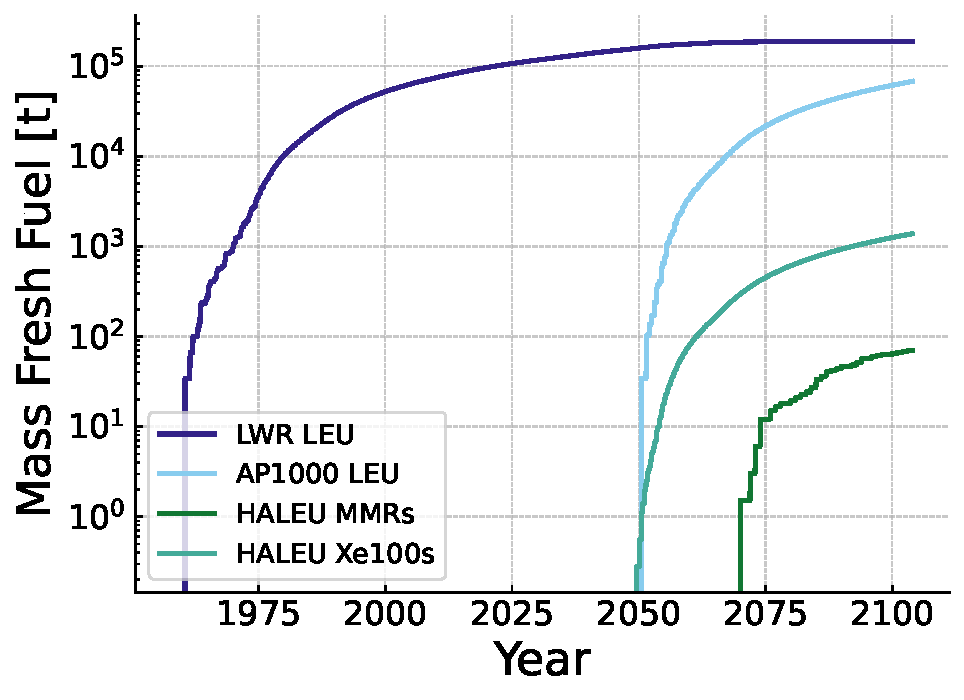
\includegraphics[width=0.495\textwidth]{images/results/used/multi_drng_used_fuel_cumulative_by_fuel.pdf}
   }
    \hfill
    \subfloat[Double. \label{fig:random_mf_d2_used}]{%
      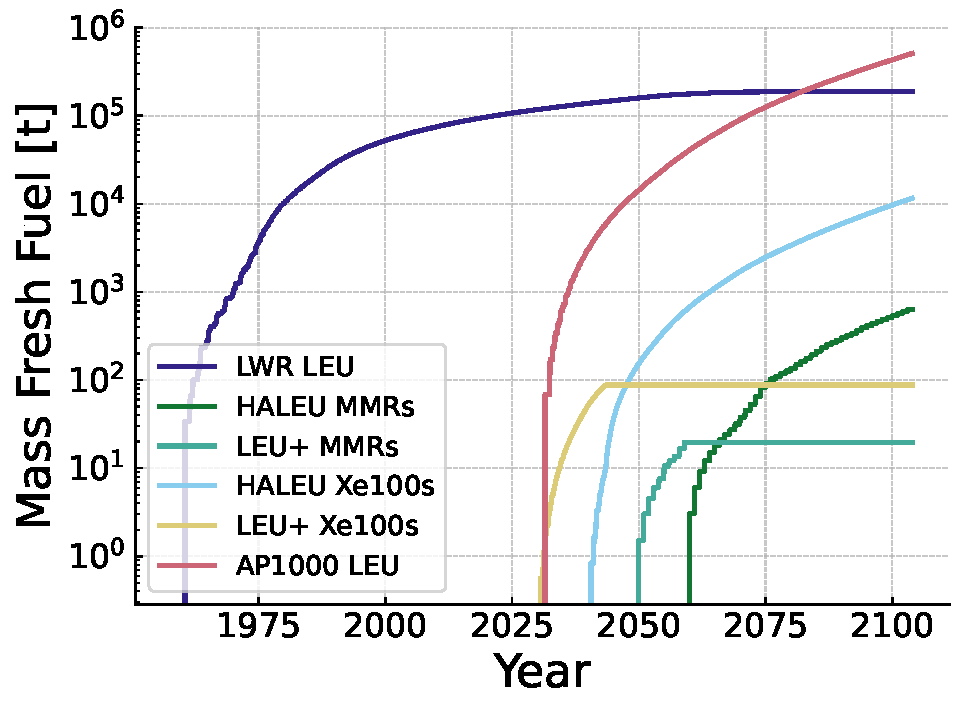
\includegraphics[width=0.495\textwidth]{images/results/used/multi_dr2_used_fuel_cumulative_by_fuel.pdf}
   }
    \caption{Random multi used fuel accumulation.}
    \label{fig:random_mf_used}
  \end{figure}


  \begin{figure}[H]
    \subfloat[No Growth. \label{fig:random_of_ng_used}]{%
      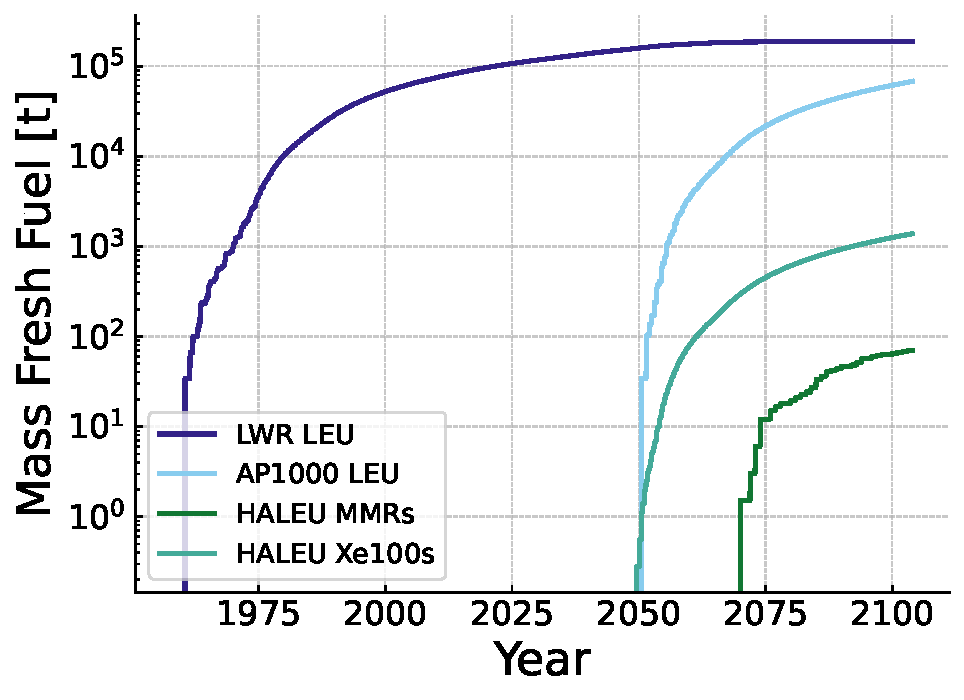
\includegraphics[width=0.495\textwidth]{images/results/used/one_drng_used_fuel_cumulative_by_fuel.pdf}
   }
    \hfill
    \subfloat[Double. \label{fig:random_of_d2_used}]{%
      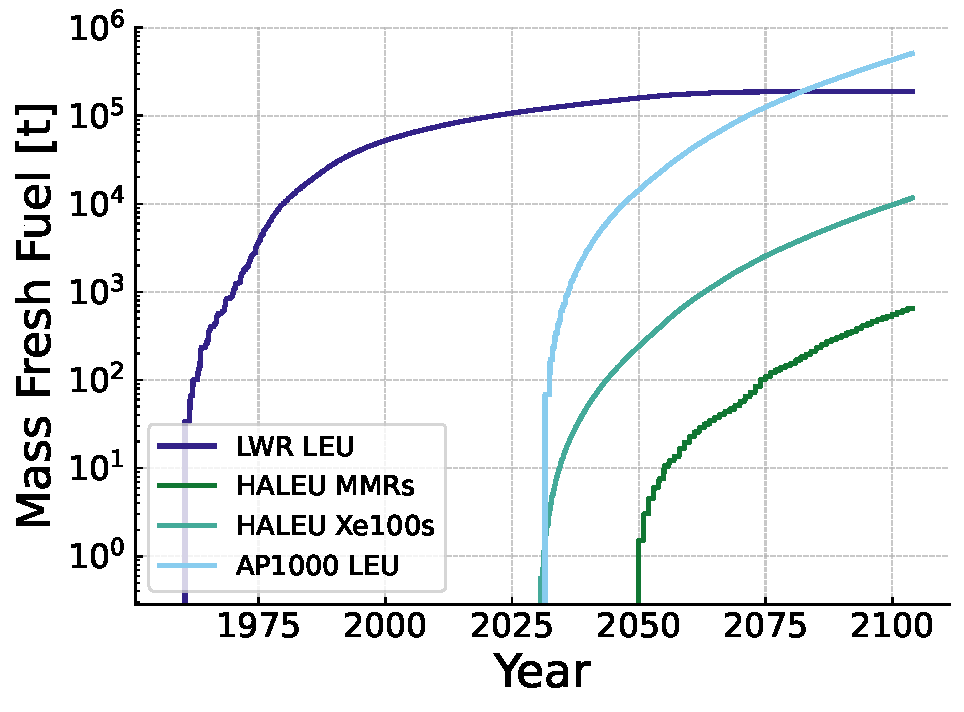
\includegraphics[width=0.495\textwidth]{images/results/used/one_dr2_used_fuel_cumulative_by_fuel.pdf}
   }
    \caption{Random single used fuel accumulation.}
    \label{fig:random_of_used}
\end{figure}


Table \ref{tab:random_used_avg} shows the average total yearly used fuel for the \textit{no growth} and \textit{double by 2050} scenarios in the single and multi-fuel enrichment deployments under the random deployment scheme. The \gls{xe} reactors show a 742\% increase in the average total yearly used fuel from the \textit{no growth} scenario to the \textit{double by 2050} scenario in the single-fuel enrichment deployment. The \gls{mmr} reactors show a 838\% increase in the average total yearly used fuel from the \textit{no growth} scenario to the \textit{double by 2050} scenario in the single-fuel enrichment deployment. The AP1000 reactors show a 649\% increase in the average total yearly used fuel from the \textit{no growth} scenario to the \textit{double by 2050} scenario in the single-fuel enrichment deployment.

\begin{table}[H]
    \centering
    \caption{Average random yearly used fuel by design in tonnes.}
    \label{tab:random_used_avg}
    \begin{tabular}{l c c c c}
       \toprule
       Scenario & \shortstack{No Growth,\\ Single} & \shortstack{No Growth,\\ Multiple} & \shortstack{Double,\\ Single} & \shortstack{Double,\\ Multiple}  \\
       \midrule
       \gls{mmr} \gls{haleu}   & \textcolor{white}{00}0.077    & \textcolor{white}{00}0.077   & \textcolor{white}{00}0.722    & \textcolor{white}{00}0.700    \\
       \gls{mmr} \gls{leup}    & --       & --      & --       & \textcolor{white}{00}0.107    \\
       \gls{xe} \gls{haleu}    & \textcolor{white}{00}1.536    & \textcolor{white}{00}1.536   & \textcolor{white}{0}12.930   & \textcolor{white}{0}12.833   \\
       \gls{xe} \gls{leup}     & --       & --      & --       & \textcolor{white}{00}0.022    \\
       AP1000 \gls{leu}        & \textcolor{white}{0}75.638   & \textcolor{white}{0}75.638  & 566.239  & 566.239  \\
       \bottomrule
    \end{tabular}
\end{table}

% talk about repositories